% !TEX encoding = UTF-8 Unicode
\title{Solana:\\
高パフォーマンスなブロックチェーンを実現する\\
新しいアーキテクチャ v0.8.13 }

\author{
        Anatoly Yakovenko \\
        anatoly@solana.io\\
}
\date{}

\documentclass[12pt]{ltjsarticle}

% \usepackage{draftwatermark}
% \SetWatermarkText{Confidential}
% \SetWatermarkScale{5}
% \SetWatermarkColor[gray]{0.95}

\usepackage{graphicx}
\usepackage{bytefield}
\usepackage{makecell}

\usepackage[]{hyperref}
\hypersetup{
    pdftitle={Solana: A new architecture for a high performance blockchain},
    pdfauthor={anatoly@solana.io},
    pdfsubject={blockchain},
    pdfkeywords={blockchain, bitcoin, cryptocurrency},
    bookmarksnumbered=true,     
    bookmarksopen=true,         
    bookmarksopenlevel=1,       
    colorlinks=true,            
    pdfstartview=Fit,           
    pdfpagemode=UseOutlines,    % this is the option you were lookin for
    pdfpagelayout=TwoPageRight
}

\begin{document}
\maketitle

\textbf{\footnotesize 免責事項}\scriptsize
~~当資料はトークンの販売を意図した文書ではなく、Solanaの仕組みに対する読者からのフィードバックやコメントを集めることを目的としたものである。Solanaがトークンセール(SAFT形式等)を開催する場合には、リスク要因など開示すべき情報をまとめた文書を作成する。その際は併せて本文の最新版が開示される予定だが、大幅な改訂がなされる可能性がある。また米国内に向けて販売がおこなわれる場合は、認定投資家のみを勧誘対象とする予定である。

本文はSolanaの事業やトークンの発展性、利用価値、金銭的価値を確約したものではない。このホワイトペーパーに記載される内容は現時点における予定を記したもので、それはプロジェクトの方針により変更されうる。またデータ、暗号通貨の市況やその他の要因、つまりSolanaプロジェクトが持つ影響力の範疇を超えたことに起因して、この目論見の成否に影響を与えることも予想される。本文中の未来事象に関する記述はSolanaプロジェクトの分析に基づいたものであり、その見込みは確約されたものではない。

\begin{abstract}
本文ではProof of History(PoH)による新たなブロックチェーンのアーキテクチャを提言する。PoHはトラストレスなネットワークにあって、一連のイベント発生タイミングの前後関係を記帳し、それを証明する仕組みである──この台帳の特徴は、情報を追記することは可能だが、記帳済みの情報の書き換えは不可能である。PoHはProof of Work(PoW)あるいはProof of Stake(PoS)などの合意形成アルゴリズムと併用することで、Byzantine Fault Tolerantによるステートマシーンの状態共有のオーバーヘッドを低減し、結果的に合意形成にかかる時間を短縮することができる。またPoHによる時間管理の性能をより強固にする二つのアルゴリズムを紹介する。ひとつは任意のサイズに分断されたネットワークから復旧可能なPoSアルゴリズム、もうひとつはProof of Replication(PoRep)を効率的にストリーミングするアルゴリズムである。PoRepとPoHの組み合わせは、時間(順序)とデータ保管を司る台帳の偽造に対する防衛手段となる。現代のハードウェア性能と1Gbpsのネットワーク環境が備えられていることを前提として、このプロトコルによる実装は最大710,000TPS(transaction per-second)のスループットが実現可能であることを示す。
\end{abstract}


\section{はじめに}\normalsize
ブロックチェーンは耐障害性を備える複製されたステートマシンの実装である。現在パブリックに利用可能なブロックチェーンの生成アルゴリズムは時間に依存しない、あるいはネットワーク参加者が正確な時間を管理できていることに期待しない\cite{tendermint,hashgraph}。ネットワーク上の各ノードはローカル時間のみを参照し、他ノードのローカル時間をまったく意識しない。『信頼できる時間の基準がない』ということは、タイムスタンプをメッセージの承諾・拒否の判断に用いる場合に、すべてのノードがそのメッセージに対する判断を同じように下すとは限らないということになる。ここで紹介するPoHは、ネットワーク上の時間の基準となりえる台帳を提供する設計になっている。ここでいう時間とは、二つのイベントに挟まれた期間やメッセージの順序関係を指す。ネットワーク上のすべてのノードは、そのネットワークがトラストレスであるにも関わらず、PoHが生成した時間の基準に依拠できるようになると期待される。
\section{本文の構成}
本資料は次のような構成が取られている。セクション\ref{design}ではシステム設計の全体像が描かれている。セクション\ref{proof_of_history}ではProof of Historyの詳細が語られている。セクション\ref{proof_of_stake}では今回提案されるProof of Stakeによる合意形成アルゴリズムが示されている。セクション\ref{porep}では高速なProof of Replicationの仕組みが詳細に説明されている。セクション\ref{system_architecture}ではシステムアーキテクチャとパフォーマンス上限に関する分析がなされている。セクション\ref{sec:smartcontracts}ではGPU計算向きの高パフォーマンスなスマートコントラクト・エンジンについて詳しい考察がなされている。

\section{ネットワークデザイン}\label{design}

\begin{figure}[h]
  \begin{center}
    \centering
    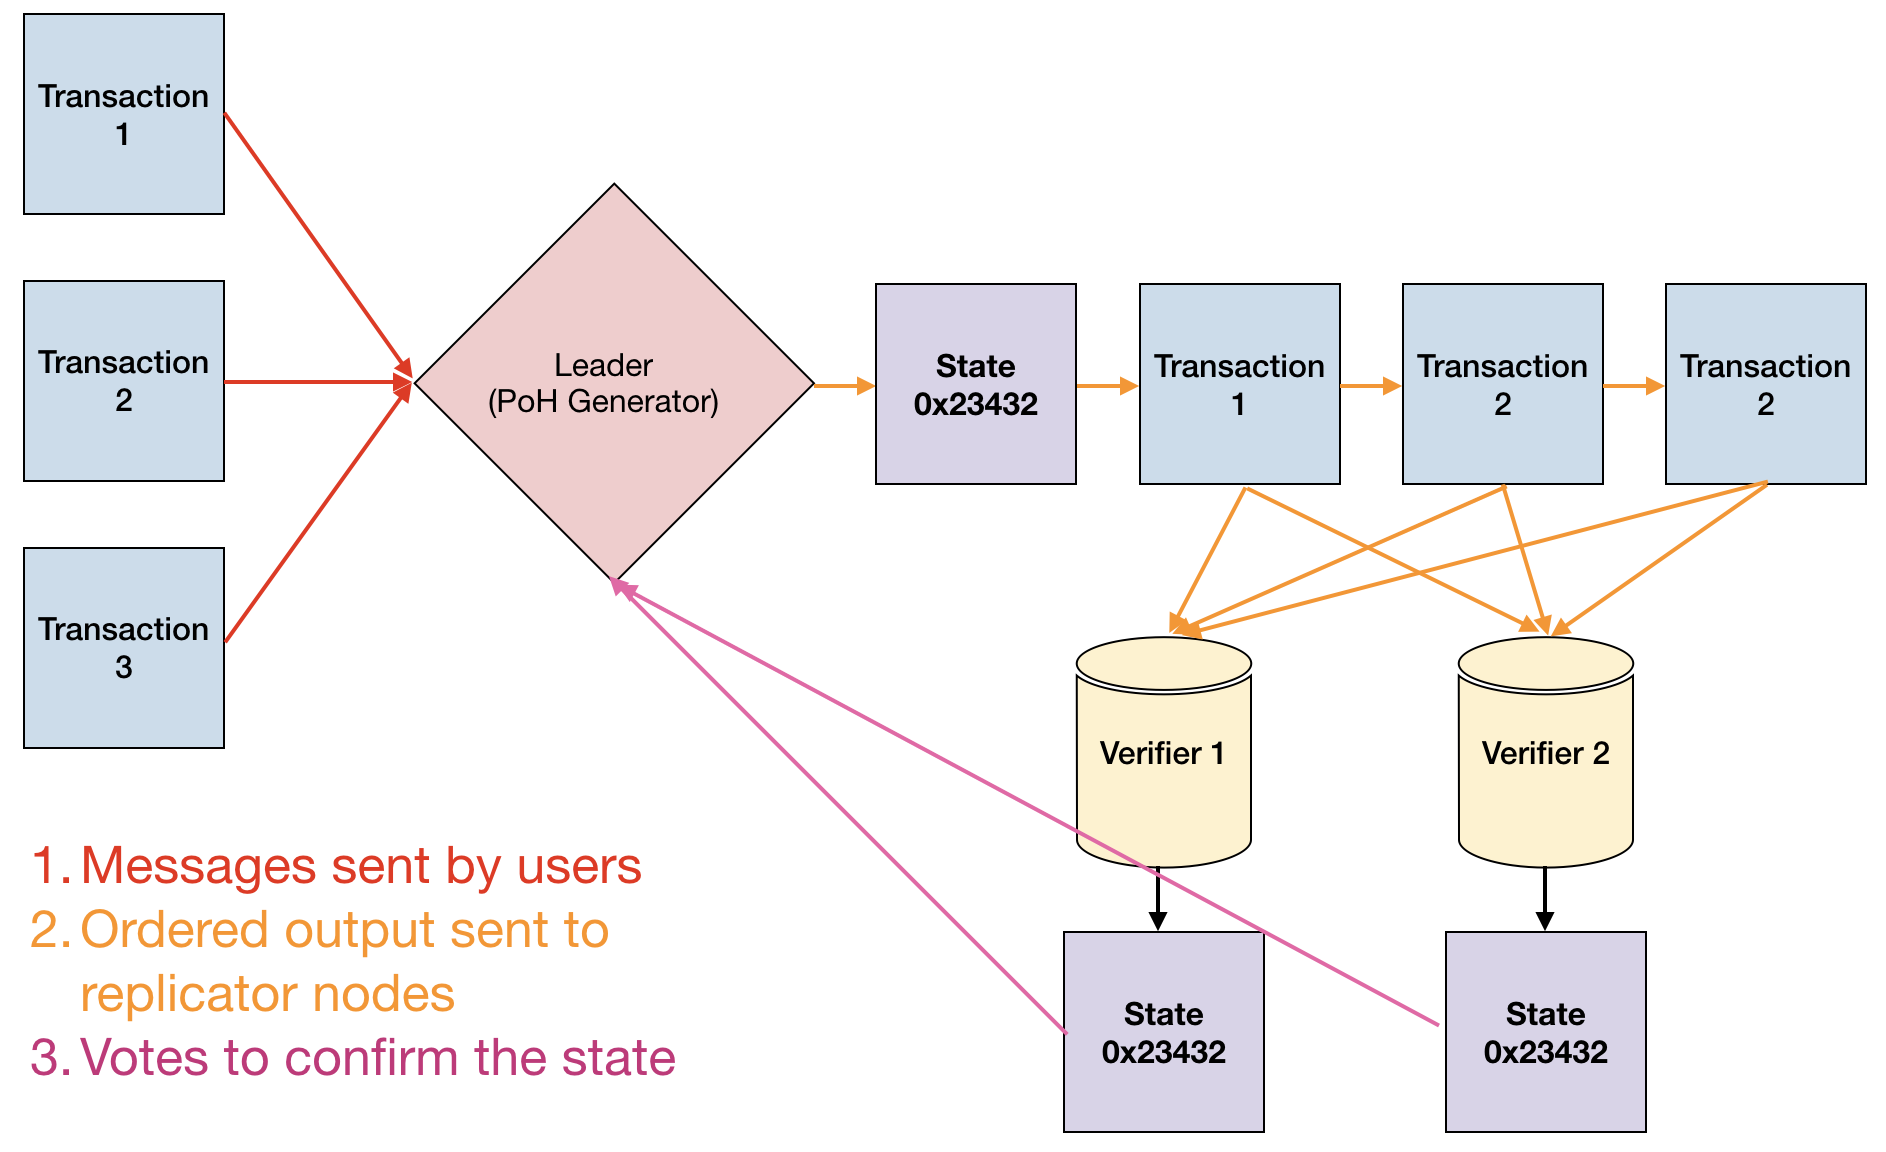
\includegraphics[width=\textwidth]{../../figures/network_design_001.png}
    \caption[Fig 1]{ネットワーク上のトランザクションフロー\label{fig:design}}
  \end{center}
  \end{figure}

図\ref{fig:design}に示されているように、システムノードは常にLeaderとしてProof of Historyの生成を担う。これはネットワーク全体で一貫性のある時間軸を提供する。スループットを最大化するため、他ノードが効率よく処理を進められるよう、Leaderはユーザメッセージを並べて順序付けする。これはRAM(主記憶装置)に格納された状態に基づいてトランザクションを執行し、実行結果を署名付きでVerifierと呼ばれるノードに引き渡す。Verifierは各自がRAM上に保持している状態から同じトランザクションを繰り返し、実行結果を確認してそれに署名を付与する。この署名付きの計算結果は票となり、ネットワーク上の正史を選び出すための合意形成アルゴリズムに用いられる。

ネットワークが分断されていない状況下では、常にLeaderはネットワーク上にひとつ存在する。各VerifierノードはLeaderと同性能のハードウェアを備えるようにし、PoSに基づいてLeaderとして選出される可能性が与えられる。ここで挙げられたPoSのアルゴリズムはセクション\ref{subsec:elections}で詳しく説明する。

ネットワークの分断が発生してしまった場合、CAP定理に基づくと一貫性は可用性より優先される。大規模な分断が発生する状況を想定して、本資料は任意のサイズで分断された状態からネットワークを復旧させるメカニズムを説明する。詳細はセクション\ref{availability}を参照されたい。

\section{Proof of History}\label{proof_of_history}

Proof of Historyは任意の二つのイベントに挟まれた時間の経過を暗号学に検証できる方法を提供する。これには入力から出力を予測することが不可能な暗号学に安全な関数で計算することが求められる。一連の計算は単一コア上で行われ、前回計算のアウトプットは今回計算のインプットとして使われる。関数が呼び出される度、その計算結果と呼び出し回数を記録する。ここまで行われた計算の入出力を分割して、外部マシンの複数コアに並列で再計算させることで、計算結果に対する正否の検証が行われる。
データそのもの、あるいはデータのハッシュ値をシーケンスに加えることは、タイムスタンプに相当する情報をそのデータに付与することにあたる。つまりそれは状態、順序、データの記録が、次のハッシュ計算が開始された以前に完了していたことの証明に他ならないからだ。この設計は、複数のシーケンス生成者同士が互いのシーケンスに含まれる情報を提供し、その情報を計算のインプットとして混ぜ込み、同期を取ることができる平行スケーリングをサポートする。この平行スケーリングについてはセクション\ref{poh:scale}で少し踏み込んだ議論を行う。

\subsection{概要説明}
システムは次のように設計される。実行前に計算結果を予測できない暗号学的ハッシュ関数(例:\texttt{sha256}、\texttt{ripemd}など)を用いる。無作為に選ばれた値を初期入力値としてハッシュ計算を開始、今回の計算結果を次回計算の入力値として使う。今回計算も次回計算も実行するハッシュ関数は同じである。関数の呼び出し回数および計算結果は順次記録される。またここで登場した初期入力値は、当日のニューヨークタイムズ紙の見出しなど、任意の文字列を選択して良い。
\\\\
\begin{center}
  \begin{tabular}{  l  l  r }
%    \hline
    \multicolumn{3}{c}{PoHシーケンス} \\
    \hline
    順番  & 計算内容 & 計算結果 \\ \hline
    $1$ & sha256(\char`\"無作為に選ばれた初期入力値\char`\") & \texttt{hash1}\\ %\hline
    $2$ &  sha256(\texttt{hash1}) & \texttt{hash2}\\ %\hline
    $3$ & sha256(\texttt{hash2}) & \texttt{hash3}\\ %\hline
    \end{tabular}
\end{center}

\noindent 図中の\texttt{hashN}はN番目に行われたハッシュ計算の結果を表している。\\

ここで要求されるのは都度ハッシュ計算結果と順序番号を発行することに尽きる。\\

\begin{center}
  \begin{tabular}{ l  l  r }
    \multicolumn{3}{c}{PoHシーケンス} \\
    \hline
    順番  & 計算内容 & 計算結果 \\ \hline
    $1$ & sha256(\char`\"無作為に選ばれた初期入力値\char`\") & \texttt{hash1}\\
    $200$ &  sha256(\texttt{hash199}) & \texttt{hash200}\\
    $300$ & sha256(\texttt{hash299}) & \texttt{hash300} \\
    \end{tabular}
\end{center}

ハッシュ関数に衝突耐性が備わっている限り、この一連のハッシュ値はシングルスレッドのみで計算可能である。これは$300$番目のハッシュ計算結果は、当該ハッシュ計算を$300$回繰り返すまで求まらないことから明らかである。この制約から$0$番目から$300$番目までの計算が終わるまでには相応の時間が経過していることが分かる。

図\ref{fig:poh_seq}中にあるハッシュ値\texttt{62f51643c1}は$510144806912$番目に求められ、ハッシュ値\texttt{c43d862d88}は$510146904064$番目に求められたことを表している。既に説明した通り、$510144806912$番目と$510146904064$番目の間にかかった計算時間の分だけ現実世界の時間も経過することがわかる。

\begin{figure}[h]
  \begin{center}
    \centering
    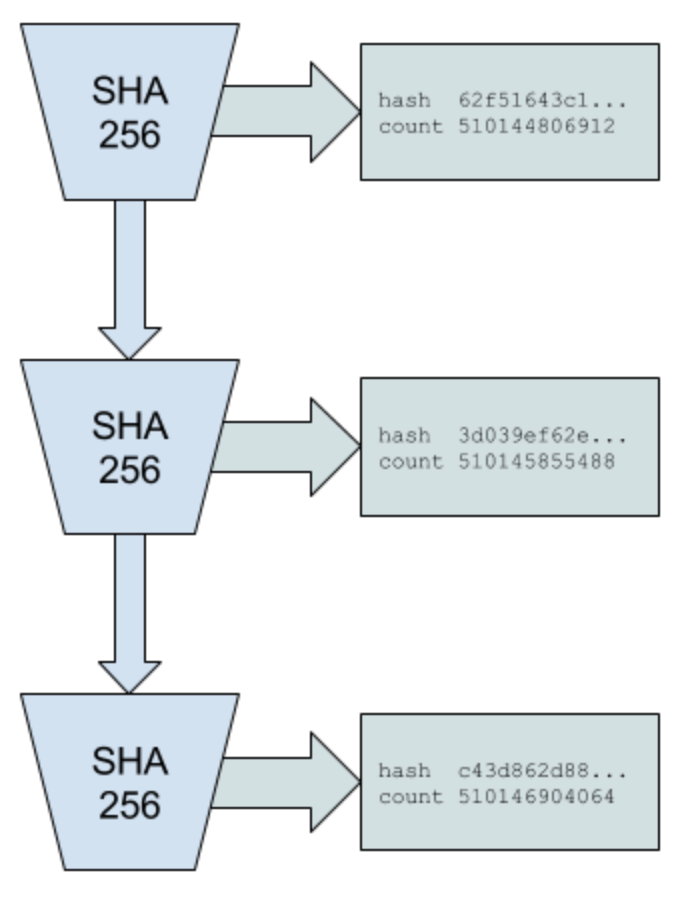
\includegraphics[width=0.5\textwidth]{../../figures/poh_sequence_001.png}
    \caption[Figure 2]{Proof of Historyシーケンス\label{fig:poh_seq}}
  \end{center}
  \end{figure}

\subsection{イベントのタイムスタンプ}

上述の通り、このハッシュ値のシーケンスは、あるデータがシーケンスに挿入される以前に、対象のデータが作成されていたことの記録として用いることができる。それはデータと現在の順序に弾き出されて来たハッシュ値に「combine」関数を適用することで、順序と値が組み合わされた計算結果が記録として残るためである。このとき任意のイベントデータが暗号学的にユニークなハッシュ値に変換される。combine関数は常に衝突耐性を備え、単純に計算結果を積み重ねていくことができる。結果的に得られたハッシュ値はそのデータにとってのタイムスタンプとなる。それは以前のハッシュ値を基にして生成されたハッシュ値であるため、以前に記録されたデータよりも後に生成されていることが言えるからである。\\

\begin{center}
  \begin{tabular}{ l l r }
    \multicolumn{3}{c}{PoHシーケンス} \\
    \hline
    順番  & 計算内容 & 計算結果 \\ \hline
    $1$ & sha256(\char`\"無作為に選ばれた初期入力値\char`\") & \texttt{hash1}\\
    $200$ & sha256(\texttt{hash199}) & \texttt{hash200}\\ 
    $300$ & sha256(\texttt{hash299}) & \texttt{hash300}\\ 
    \end{tabular}
\end{center}


\noindent 例えば写真撮影など、なにか電子データが作成されるようなイベントが発生したとき、\\\\\noindent
\begin{center}
  \begin{tabular}{ l l r}
    \multicolumn{3}{c}{データを含むPoHのシーケンス} \\
    \hline
    順番  & 計算内容 & 計算結果 \\ \hline
    $1$ & sha256(\char`\"無作為に選ばれた初期入力値\char`\") & \texttt{hash1}\\
    $200$ & sha256(\texttt{hash199}) & \texttt{hash200} \\ 
    $300$  & sha256(\texttt{hash299}) & \texttt{hash300}\\ 
    $336$ & sha256(append(\texttt{hash335}, 撮影データのsha256値)) & \texttt{hash336}\\ 
    \end{tabular}
\end{center}


\texttt{Hash336}は\texttt{hash335}と撮影データの\texttt{sha256}値を入力値として計算されている。こうして撮影データの\texttt{sha256}値とその順番はシーケンスに記録される。つまり入力値さえ特定できていれば、誰でもこのシーケンスに対する変更内容を再現して検証することができるのだ。シーケンス上の各部分は並列で検証できることになるが、詳しくはセクション\ref{poh:verify}で説明する。

一連の計算はひとつずつ順番に行わざるを得ない仕組みから、ある情報がシーケンスに挿入されたタイミングは、それ以降に計算されたハッシュ計算が完了するより以前であることを明らかにできる。

\begin{center}
  \begin{table}
  \begin{tabular}{l l r}
    \multicolumn{3}{c}{POHシーケンス} \\ \hline
    順番  & 計算内容 & 計算結果 \\ \hline
    $1$ & sha256(\char`\"無作為に選ばれた初期入力値\char`\") & \texttt{hash1}\\
    $200$ & sha256(hash199) & \texttt{hash200} \\ 
    $300$ & sha256(hash299) & \texttt{hash300} \\ 
    $336$ & sha256(append(hash335, 撮影データ1のsha256値)) & \texttt{hash336}\\ 
    $400$ & sha256(hash399) & \texttt{hash400} \\ 
    $500$ & sha256(hash499) & \texttt{hash500}\\ 
    $600$ & sha256(append(hash599, 撮影データ2のsha256値)) & \texttt{hash600}\\ 
    $700$ & sha256(hash699) & \texttt{hash700}\\ 
    \end{tabular}
    \caption[Table 1]{2つのイベントを挿入したPoHシーケンス\label{table:multievent}}
    \end{table}
\end{center}

表\ref{table:multievent}のシーケンスから\texttt{撮影データ2}が\texttt{hash600}の計算完了より以前に、\texttt{撮影データ1}が\texttt{hash336}の計算完了より以前に作成されたことが分かる。ハッシュ値をシーケンスに書き込むことは、結果的に後続すべての計算結果に影響を与えることになる。シーケンスへ挿入したいデータに適用されるハッシュ関数が衝突耐性を備える限り、今後どのようなデータが追加されるか分かっていたとしても、未来のシーケンスを事前に予測することは不可能である。\\

シーケンスに挿入されるデータは無加工でも、メタデータ付きハッシュ値でも良い。\\

\begin{figure}[h]
  \begin{center}
    \centering
    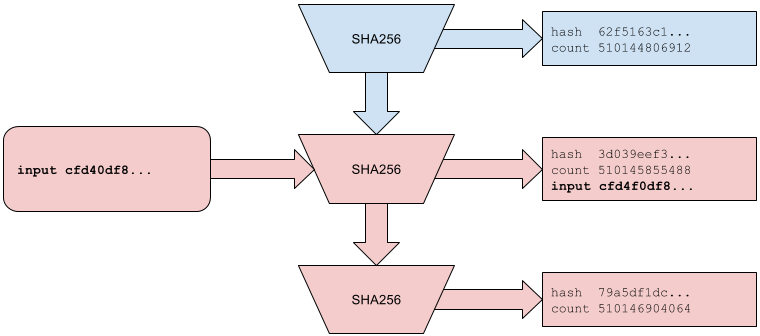
\includegraphics[width=0.9\textwidth]{../../figures/fig_3.png}
    \caption[Fig 3]{Proof of Historyへのデータの挿入\label{fig:poh_insert}}
  \end{center}
  \end{figure}

  図\ref{fig:poh_insert}では入力値\texttt{cfd40df8\ldots}がProof of Historyのシーケンスへ挿入されている。挿入された順番は$510145855488$で、その時点の状態は\texttt{3d039eef3}である。将来生成されるすべてのハッシュ値は、今回のシーケンスに対するデータ挿入により影響を受ける。その影響範囲を図中では色付きで表現している。\\\\

シーケンスを観察しているノードは、すべてのイベントが挿入された順序と、任意のふたつの挿入時点の間で経過した時間を見積もることができる。

\subsection{検証}\label{poh:verify}
検証時の計算はマルチコアで実行可能なので、生成時よりも圧倒的に短い時間で完了することができる。\\

\begin{center}

\begin{tabular}{l l r}
    \multicolumn{3}{c}{コア1} \\ \hline
    順番  & 計算内容 & 計算結果 \\ \hline
    $200$ & sha256(\texttt{hash199}) & \texttt{hash200} \\ 
    $300$ & sha256(\texttt{hash299}) & \texttt{hash300}\\ 
    \end{tabular}\\
    
  \begin{tabular}{l l r}
    \multicolumn{3}{c}{コア2} \\
    \hline
    順番  & 計算内容 & 計算結果 \\ \hline
    $300$ & sha256(\texttt{hash299}) & \texttt{hash300} \\
    $400$ & sha256(\texttt{hash399}) & \texttt{hash400}\\ 
    \end{tabular}
    
\end{center}


例えば$4000$コアを備えるGPUを使って計算する場合、検証者は生成されたシーケンスを$4000$に分割して、先頭から末尾までのハッシュ計算が正しく行われていたかを並列計算で確認できる。シーケンス生成にかかる計算時間を次のように計算できるとすると、\\


\[
\frac{\textrm{ハッシュ計算の総回数}}{\textrm{1コアで処理される秒間ハッシュ計算回数}}
\]

\noindent 検証にかかる計算時間は、\\

\[
\frac{\textrm{ハッシュ計算の総回数}}{\textrm{(1コアで処理される秒間ハッシュ計算回数 * 検証に使えるコア数)}}
\]

\begin{figure}
  \begin{center}
    \centering
    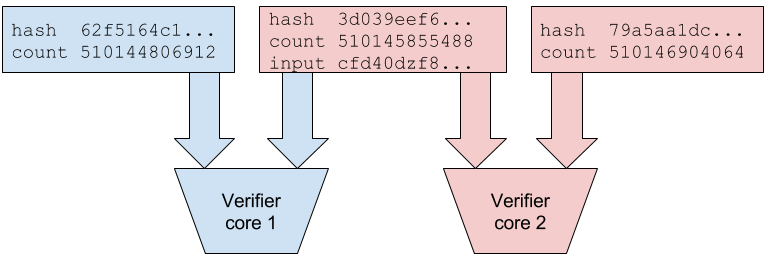
\includegraphics[width=0.9\textwidth]{../../figures/fig_4.png}
    \caption[Figure 4]{複数コアによる検証\label{fig:poh_verify}}
  \end{center}
  \end{figure}

図\ref{fig:poh_verify}では分割されたシーケンスを各コアが並列で検証している。すべてのインプットは順番と状態と併せて計算結果に記録され、検証者は同じ計算を繰り返すことでシーケンスを複製していく。赤色に染められたハッシュ値は、シーケンスがデータ挿入により変更されたことを指している。

\subsection{平行スケーリング}\label{poh:scale}
複数のProof of History生成者同士でシーケンスの状態を共有することで、平行スケーリングの実現を可能とする。このスケーリングはシャーディングを使わずに果たせる。2つの生成者でスケーリングする場合、双方のシーケンスに記録されている全てのイベントの順序を分かるフルシーケンスを構築するためには、各生成者が導き出した計算結果が必要となる。

\begin{center}
  \begin{tabular}{|l c r|}

  \hline
    \multicolumn{3}{|c|}{PoH生成者A} \\
  %  \hline
    順番  & ハッシュ値 & データ \\ \hline
    $1$ & \texttt{hash1a} & \\ 
    $2$ & \texttt{hash2a} & \texttt{hash1b} \\ 
    $3$ & \texttt{hash3a} & \\ 
    $4$ & \texttt{hash4a} & \\
    \hline
    \end{tabular}
  \begin{tabular}{| l  c  r |}
  \hline
    \multicolumn{3}{|c|}{PoH生成者B} \\
%    \hline
    順番  & ハッシュ値 & データ \\ \hline
    $1$ & \texttt{hash1b} & \\ 
    $2$ & \texttt{hash2b} & \texttt{hash1a} \\ 
    $3$ & \texttt{hash3b} & \\ 
    $4$ & \texttt{hash4b} & \\
    \hline
    \end{tabular}
\end{center}

図中のように生成者AとBが参加している場合、AはBから直近の状態をデータパケット(hash1b)として受け取る。生成者Aが次に取る状態のハッシュ値は、生成者Bから提供された状態を含めて計算される。よってhash1bはhash3aより以前に計算済みであったことを示すことができる。この仕組みは、例えば3つ生成者が存在しているとき、\(A \leftrightarrow B \leftrightarrow C\)のように1組(AとC)が直接同期を取っていなくてもA、B、C間のフルシーケンスを求めることは可能である。

定期的に同期することで、各生成者は外部のトラフィックを処理することが可能となり、システム全体として対処可能なイベント数を増幅させることができるようになる。ただしネットワークを通した同期であるため、生成者間で生じるレイテンシ分だけ時間の計測精度が犠牲となる。この同期中に発生するグローバルな順序決定の問題は、ハッシュ値順にするなどの事前に取り決めた方法で順序を決定づける。

\begin{figure}
  \begin{center}
    \centering
    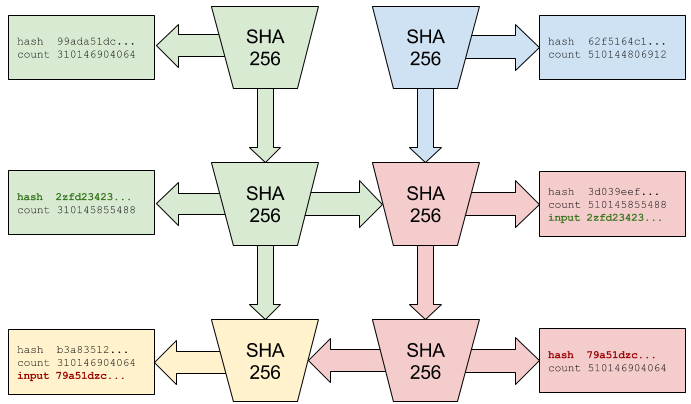
\includegraphics[width=0.9\textwidth]{../../figures/fig_5.png}
    \caption[Fig 5]{同期する二つの生成者\label{fig:poh_scale}}
  \end{center}
  \end{figure}

図\ref{fig:poh_scale}は二つの生成者が出力した状態を共有し合い、互いのシーケンスに挿入している様子を表している。色の変化は同期によりシーケンスに影響を受けたことを表現している。同期時に共有されたハッシュ値は色付きの太字で表現されている。

この同期方法により、\(A \leftrightarrow B \leftrightarrow C\)のように直接同期していない生成者同士でも、三者間のイベント順序は矛盾なく決定することができる。

%%It is worth noting that the theoretical $710$k tx/s on a $1$~gb network based on the PoH design does not account for additional capacity offered through  horizontal scaling.
このスケーリング方法は回線稼働率が枷になる。$10 \times 1$~gbpsの回線で構成されるネットワーク環境では、回線稼働率が0.999のとき、ネットワーク全体の回線稼働率は\(0.999^{10} = 0.99 \)となる。

\subsection{一貫性}
生成済みのシーケンス上の最後の計算結果を次回計算の入力値にすることで、一貫性と攻撃耐性が維持されると期待される。\\

\begin{center}
  \begin{tabular}{ | l c r |}
    \hline
    \multicolumn{3}{|c|}{PoHシーケンスA} \\
    順番 & データ & 計算結果ハッシュ値  \\ \hline
    $10$ & & \texttt{hash10a} \\ 
    $20$ & Event1 & \texttt{hash20a} \\ 
    $30$ & Event2 & \texttt{hash30a} \\ 
    $40$ & Event3 & \texttt{hash40a} \\
    \hline
    \end{tabular}
  \begin{tabular}{ | l c r |}
    \hline
    \multicolumn{3}{|c|}{PoH隠れシーケンスB} \\
    順番 & データ & 計算結果ハッシュ値  \\ \hline
    $10$ & & \texttt{hash10b}\\ 
    $20$ & Event3 & \texttt{hash20b}  \\ 
    $30$ & Event2 & \texttt{hash30b} \\ 
    $40$ & Event1 & \texttt{hash40b} \\
    \hline
    \end{tabular}
\end{center}

悪意を持ったPoH生成者はイベントの発生順序を変えた隠れシーケンスを作る可能性がある。発生するイベントの情報へすぐにアクセスできるなら、正しいシーケンスよりも素早く隠れシーケンスを生成することも可能である。\\

この攻撃を防ぐために、クライアントがイベントを送信するときは、クライアント自身が正規であると認識するシーケンス上の最新ハッシュ値を送信内容に含めることを求められる。クライアントがEvent1を作成するとき、それに最新ハッシュ値を付与する必要がある。\\

\begin{center}
  \begin{tabular}{  l  c l}

    \multicolumn{3}{c}{PoHシーケンスA} \\
    \hline
    順番  & データ & 計算結果ハッシュ値 \\ \hline
    $10$ & & \texttt{hash10a} \\ 
    $20$ & Event1 = append(event1 data, \texttt{hash10a}) & \texttt{hash20a}  \\ 
    $30$ & Event2 = append(event2 data, \texttt{hash20a}) & \texttt{hash30a} \\ 
    $40$ &  Event3 = append(event3 data, \texttt{hash30a}) & \texttt{hash40a} \\
    \end{tabular}
\end{center}

シーケンス発行時にEvent3がhash30aを参照しているとき、そのハッシュ値がイベント発生以前に存在しない場合に、シーケンス利用者は参照先のシーケンスに異常を検知する。こうして一部分のイベント順序を書き換える攻撃が有効になるのは、クライアントがイベント送信前に検知したハッシュ値の順番から、そのイベント情報はシーケンスに挿入されるまでの間だけに制限される。つまり極めて短期間の間に発生したイベントの前後関係に影響受けない問題を解決するクライアントソフトウェアに絞って利用することが望ましい。

悪意のあるPoH生成者がクライアント側で付与したハッシュ値を書き換えることを防ぐため、クライアントはイベントデータとハッシュ値に署名を付与した上で送信を行う。\\
\begin{center}
  \begin{tabular}{  l  l  r }
    \multicolumn{3}{c}{PoHシーケンスA} \\
    \hline
    順番  & データ & 計算結果ハッシュ値 \\ \hline
    $10$ & & hash10a  \\ 
    $20$ & \makecell{Event1 = sign(append(event1 data, hash10a), \\利用者の秘密鍵)} & hash20a\\ 
    $30$ & \makecell{Event2 = sign(append(event2 data, hash20a), \\利用者の秘密鍵)} & hash30a \\ 
    $40$ & \makecell{Event3 = sign(append(event3 data, hash30a), \\利用者の秘密鍵)} & hash40a \\

    \end{tabular}
\end{center}

このデータの検証を行うためには、署名と付与されたハッシュ値がシーケンス上で保たれていることが必要とされる。\newpage
\noindent 検証方法:\\

\noindent\texttt{(Signature, PublicKey, hash30a, event3 data) = Event3} \\
\texttt{Verify(Signature, PublicKey, Event3)}\\
\texttt{Lookup(hash30a, PoHSequence)}\\

\begin{figure}
  \begin{center}
    \centering
    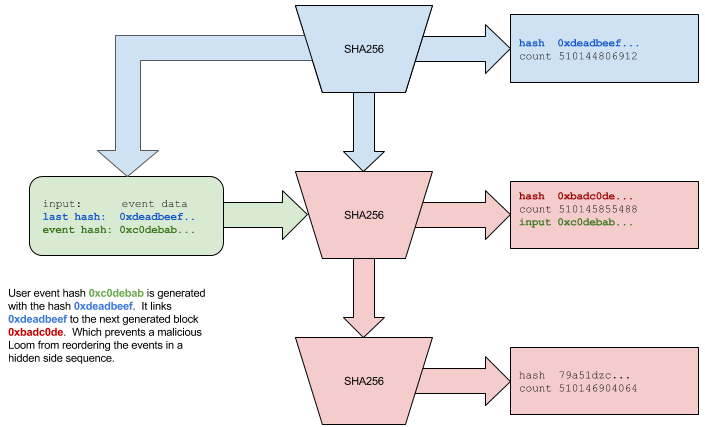
\includegraphics[width=0.9\textwidth]{../../figures/fig_6.png}
    \caption[Fig 6]{入力受付時にハッシュの存在性を検証\label{fig:poh_consistency}}
  \end{center}
  \end{figure}

図\ref{fig:poh_consistency}では、クライアントからのインプットに付与されたハッシュ値\texttt{0xdeadbeef\ldots}が、シーケンス上の遠くない過去まで遡り、それが存在していることに依存している。図上部の青い部分はクライアントが生成済みのハッシュ値を参照していることを表している。クライアントからのメッセージはハッシュ値\texttt{0xdeadbeef\ldots}を含む場合においてのみ有効とされる。図中の赤い部分はクライアントからの入力により影響を受けた箇所を指している。

\subsection{オーバーヘッド}
秒間4000回のハッシュ計算が可能な環境では、秒間160KBのデータが追加で生成され、その検証のためコア数4000のGPUを使っておよそ0.25-0.75ミリ秒のオーバーヘッドが発生する。

\subsection{攻撃}
\subsubsection{順序の逆転}
 イベントの順序を逆転させるためには、攻撃者は次のイベントを受け取った後から不正なシーケンスを生成し始めなければならない。この遅れにより、悪意のないノード同士で不正のない情報の交換が可能となる。

\subsubsection{速度}
複数の生成者が稼働することでより強力な攻撃耐性を得られる。生成者は広帯域な通信を教授でき、他の生成者と共有する状態をシーケンスに混ぜ込む機会を増やせる。また高速低帯域の生成者であっても、周期的に広帯域の生成者とイベントを混ぜ合うことができる。

こうした高速なシーケンスにより、悪意のあるノードが生成する不正なシーケンスは矯正されることになる。

\subsubsection{ロングレンジアタック}

ロングレンジアタックとは、かつて利用されていた古い秘密鍵を悪用して、不正な台帳を作ることを指す\cite{casper}。Proof of Historyはロングレンジアタックに対する防衛手段となりえる。攻撃に利用できる秘密鍵を入手した悪意のあるノードは、再作成しようとする履歴範囲の開始時点から経過したのと同程度の時間を再現する必要がある。それにはネットワーク上のノードが備える計算速度よりも高速なプロセッサを利用する必要がある。さもなくば攻撃者が作成する不正なシーケンス上で再現される時間は、正規のシーケンスには永遠に追いつくことができない。

さらに時間の基準を統一することで、Proof of Replicationの構築をよりシンプルにすることができる(詳細はセクション\ref{porep}を参照)。すべてのネットワーク参加者が一箇所のシーケンス上に記録されたイベントに依拠するためである。

PoRepとPoHを一緒に活用することで空間的にも時間的にも堅牢性を高めることができる。

\section{Proof of Stakeによる合意形成}\label{proof_of_stake}
\subsection{概要説明}
ここで取り上げるProof of Stakeは次に挙げる要件を満たすために設計されている。Proof of Historyの生成者が生み出したシーケンスを迅速に承認できること、逐次Proof of History生成者を選出できること、そして不正を働いている検証者たちへの懲罰ができること。このアルゴリズムはすべてのネットワーク参加ノードがタイムアウト発生前にメッセージを受け取れることを前提としている。
\subsection{用語の説明}
\begin{description}

\item[ボンド]
Proof of Workにおける設備コストに相当する。Proof of Workでは、採掘者はハードウェアや電気にお金を支払い、ブロックチェーンのブランチのひとつを支持する。つまりボンドとは、トランザクションを承認する権利を得るために検証者たちが担保として献上する価値のことを指す。

\item[スラッシング]

Proof of Stakeにおけるnothing at stake問題への対処法のひとつ\cite{slasher}。検証者が他のブランチを支持していたことが証明された場合、正規のブランチは検証者がステークしていた資本を処分することができる。つまり検証者の支持するブランチが発散しないよう設計された経済的インセンティブである。

\item[大多数派]
全検証者をボンドで重み付けしたときの\(\frac{2}{3}\)以上の割合を指す。大多数派からの支持によりネットワークは合意形成を完了する。つまり少なくとも\(\frac{1}{3}\)の支持を不正なブランチに流さなくては、正規ブランチへの合意形成を避けることができない。この攻撃を仕掛けるためには、通貨の時価総額の\(\frac{1}{3}\)近いコストが必要であることが示唆される。

\end{description}

\subsection{ボンディング}
ボンディングには一定量以上の通貨を必要とし、実行すると所有者に紐づく形でボンディング用の口座へ出金される。ボンディング中の残高は消費できず、所有者が引き出すまでボンディング用の口座に置かれ続ける。ボンディングされた残高は一定時間が経過するまで引き出すことはできない。ボンディング中の参加者たちから大多数の承諾を受けてボンドは有効化される。

\subsection{投票}
Proof of History生成者は、予め決められた期間の状態に対し署名を行うことができる。ボンディング中の参加者たちは各自が状態に行った署名によって、生成者の署名内容に対する承認を行わなければならない。つまり単純なYes票による投票で、否定票はない。

ボンディング中の参加者から所定時間内に大多数の支持を受けた場合、そのブランチは正式に受け入れられる。

\subsection{アンボンディング}

N票を失った通貨は枯れたものとみなされ投票に参加する権利を失う。所有者はアンボンディングの手続きを踏んで資本を取り戻すことができるようになる。

ここに挙げられたNの値は、有効票数に対し枯れた通貨量の比率により動的に変わる。Nは枯れた通貨量の増加に合わせて増えていく。これにより規模の大きいネットワークの分断が起きたとき、大きなブランチが小さなブランチよりも速く復旧する仕組みができる。

\subsection{選挙}\label{subsec:elections}
PoH生成者の選挙は生成者からエラーが検出されたときに開かれる。票をもっとも多く集めた検証者が次の生成者として選出される。同票の場合は公開鍵アドレスの値が大きい方が選択される。

新しいシーケンス開始時にはネットワークの合意が要求されるが、合意形成前にリーダーがエラーを起こした場合は、得票率が次点だった検証者が新たなリーダーとして選択される。このとき改めて合意形成を行わなければならない。

決議を変更するにはより高速なPoHシーケンス上で投票を行う必要がある。また改めて投じる票には変更前の情報を含める必要がある。これを怠るとスラッシングされる恐れがある。シーケンスへの承認が一定以上蓄積されたとき、決議の変更が可能となる。

リーダーが選出されると、その役割を引き継ぐことのできる副系を決めることができる。リーダーに異常が起きたとき副系はその役割を引き継ぎ、代わりを担う。

例外が検出された、あるいは予め定められた時点で、副系はリーダーを代わり、下位の生成者も繰り上がるような設計になる。

\subsection{選挙の開催条件}
\subsubsection{PoH生成者の分断}

PoH生成者は生成したシーケンスに署名をおこなう。PoH生成者の鍵が攻撃者に利用できる状況下においてのみ分断は発生しうる。異なるシーケンスに同じPoH生成者の署名が与えられることで分断が検知される。

\subsubsection{実行系の例外}
PoH生成者にハードウェアの誤動作やバグ、あるいは意図的に起こされたエラーにより、不正な状態や検証者の計算結果が不一致する状態が生成されることがある。これを検知した検証者はゴシップを流し、それが引き金となって新たに選挙が開催される。不正なシーケンス状態を受け入れた検証者は必ずスラッシングを受けてボンドを没収される。

\subsubsection{ネットワークのタイムアウト}

ネットワークにタイムアウトが発生した場合は選挙が開催される。

\subsection{スラッシング}
検証者が分断したシーケンス両方に票を投じるとスラッシングにより罰せられる。悪意のある投票が検知されると、ボンドされていた資本は没収されて採掘プールへ送られる。

前回分断を起こしたシーケンスへ投票していた場合でも、それは悪意のある投票とみなされず、ボンドへのスラッシングは執行されない。ただし今回分断を起こしたシーケンスへの票が無効化される。

PoH生成者が生成した不正なハッシュへ票が投じられた場合にもスラッシングが執行される。生成者は不正なシーケンス状態を無作為に発行するが、これは副系へのフォールバックを発生させる。

\subsection{副系の選挙}
副系あるいはそれ下位のProof of History生成者の選挙も開催される。選挙開催の提案はリーダー生成者のシーケンス上で行われる。タイムアウト前に合意形成がなされると副系は選出され、その役割を担う。リーダーから権限の引き渡しが行われる旨のメッセージがシーケンスに挿入される。不正な状態がシーケンスへ挿入された場合は、副系へのフォールバックが強制される。

副系が選出済みの状態でリーダーが障害を起こした場合、選挙中はその副系が最初のフォールバック先として扱われる。

\subsection{可用性}\label{availability}
分断状態になりうるCAPに基づいたシステムは、一貫性あるいは可用性のいずれかを優先しなければならない。我々のシステムは可用性を選択したが、時間の計測者という立場から、実時間に基づくタイムアウト以前においては一貫性が保たれる設計を採用する。

Proof of Stakeの承認者は一定量の通貨をステーク状態にロックアップすることで、所定の取引に投票する権利を得る。ロックアップの実施も他の取引と同様PoHのストリームに挿入される取引として扱われる。投票するためにPoS承認者は状態ハッシュ値に署名する必要がある。PoHの台帳で発生したすべての取引完了後の状態を基に、投票が行われるためである。投票の実施もPoHのストリームに挿入される。PoHの台帳をみれば、各投票がどのぐらいの時間間隔で行われていたか推測できる。分断発生時にはどのぐらいの期間、承認者たちが利用不可に陥っていたか推し測ることもできる。

分断の解決にかかる実時間を圧縮するため、利用不可に陥った承認者のステーキングを解除する動的アプローチを検討したい。ステーキングを解除された承認者は合意形成の頭数に入らないので、合意形成にかかる時間が圧縮される仕組みである。\(\frac{2}{3}\)を越える承認者が利用可能ならば合意形成に至るまでに必要なハッシュ計算回数は抑えられるため、ステーキング解除はすぐに完了できる。利用可能な承認者の割合が\(\frac{2}{3}\)以下かつ\(\frac{1}{2}\)を超えるときは、合意形成までに必要なハッシュ計算回数が増加するため、ステーキング解除にかかる時間が延びてしまう。半数以上の承認者が利用不可になる規模の大きな分断が発生した状況では、ステーキング解除の処理に多大な時間がかかる。そのような状況でも取引や投票は可能だが、\(\frac{2}{3}\)の合意形成に至るには相当数のハッシュ計算をこなし、利用不可に陥った承認者のステーキング解除が完了している必要がある。復旧にかかるネットワークの時間差は、ネットワーク利用者たちがどのパーティションを使い続けたいか選択するための猶予にあたる。

\subsection{復旧}\label{availability}
ここで紹介するシステムはどんな障害が起きても台帳を完全に復旧させることができる。つまり誰でも台帳上の任意の位置にハッシュ値や取引を追記することで分岐を作成して良い。もし分岐したシーケンス上において承認者が不在の場合、ボンドの追加がブランチ上で\(\frac{2}{3}\)の支持を集めて合意形成に至るには、極めて長い時間が必要とされる。よって検証者不在の状態から完全復旧を果たすためには相当数のハッシュ計算が台帳上で行われなければならない。つまり利用不可になった検証者全てのステーキングが解除されるまで、新たなボンドにより台帳の承認を行うことは不可能となる。

\subsection{状態確定}\label{availability}
過去に何が起きたか、それがいつ頃に起きたか照合することをPoHは可能にする。PoH生成者がメッセージストリームを流し出すごとに、承認者はその内容に署名を付けて500ミリ秒以内に提出することが求められる。この制限時間はネットワークの状況次第でさらに短縮される。その承認行為自体がストリームへ挿入されるため、投票そのものを直接観測してなかったとしても、それがタイムアウト発生前に完了していたか確認することは誰にでもできる。

\subsection{攻撃}
\subsubsection{コモンズの悲劇}
PoH生成者から流れてきた状態ハッシュ値に対してPoS承認者が検証を行わず、ひたすら承認を出し続ける状況を指す。経済的インセンティブに起因する問題である。これを回避するため、PoH生成者は無作為なタイミングで不正なハッシュを生成し、これに投票した承認者はスラッシングされる仕掛けを用意する。不正なハッシュ値が生成されたとき適切な検証と投票が行われることで、ネットワークは副系のPoH生成者へ即座に切り替えることになる。

検証者は500ミリ秒等の短い時間内に回答を返すことが求められる。悪意を持った検証者が他の検証者の投票内容を観測して、それをいち早くストリームへ挿入できてしまう確率を低減するため、タイムアウトは十分短い時間を設定される必要がある。

\subsubsection{PoH生成者との談合}\label{subsubsec:collusion}
PoH生成者と談合している承認者は、不正なハッシュが流れてくるタイミングを事前に知ることができる問題を指す。ただしこれはPoH生成者が承認者の役割も賄える通貨量以上をステーキングしていることと違いがない。結局PoH生成者は状態ハッシュ値の計算を行わなくてはならない。

\subsubsection{検閲}\label{censorship}
\(\frac{1}{3}\)のボンド保有者が新規ボンド含むシーケンスの受け入れを拒否したとき、検閲が起きているかDoSが発生していると考えられる。ここでは受け入れを拒否している\(\frac{1}{3}\)のボンド保有者を”ビザンチン・ボンド保有者”と呼ぶ。この種の攻撃に対しては、ボンドが枯れていくサイクルを動的に調整することでプロトコルは耐性を身につけることができる。DoS発生時、ビザンチン・ボンド保有者よりも規模の大きい側の保有者たちがビザンチン・ボンド保有者を検閲し、ネットワークを切り離す。これにより規模の大きい側の保有者たちは、ビザンチン・ボンドを時間経過とともに無力化していくことができるので、規模の小さい側のビザンチン・パーティションは長く生き残ることができない。

アルゴリズムは次のように動作する。多数派の合意によりリーダーが選出される。リーダーはビザンチン・ボンド保有者の参加権を取り上げる。Proof of History生成者はビザンチン・ボンド所有者の数が十分に減り、多数派の割合が大多数派の規模に至るまでの経過時間を記録するためシーケンス生成を継続する。どの程度のボンドが有効化されているかに依って、ボンドが枯れていく速度が動的に決まる。そして分岐した少数派のネットワークは、多数派のネットワークが大多数派に格上げされるまで以上の長い時間を待たされることになる。大多数派が成立したとき、ビザンチン・ボンド保有者にスラッシングの罰を下すことができる。

\subsubsection{ロングレンジアタック}\label{censorship}
PoHは本質的にロングレンジアタックに対する耐性を持つ。過去の一時点からロングレンジアタックを試みる攻撃者は、PoH生成者の計算能力を越える速度で計算しない限り、永遠に正規台帳を差し替えることはできない。

合意形成プロトコルは第二の防壁である。これは如何なる攻撃も全検証者をステーク解除するより長い時間をかける必要があるためである。これは台帳の履歴に刻まれる可用性に”差”を生み出す要因ともなる。つまり二つの台帳を同じハッシュ計算回数時点で比べた時、最大断片数が最小の台帳が正規のものと考えることができる。

\subsubsection{ASIC攻撃}\label{censorship}

このプロトコルではASICによる攻撃のタイミングが二つ存在する──ネットワーク分断時と状態確定時における作為的タイムアウトである。

分断時のASIC攻撃については、ステーキング解除速度が非線形であり、大規模な分断を起こしているネットワークでは圧倒的に遅いオーダーを弾き出すため、ASICを用いるメリットが極めて低い。

状態確定時のASIC攻撃については、ビザンチン側の検証者たちにボンドのステーキング承認待ちを許し、協力者のPoH生成者を使って投票内容をねじ込めてしまうという弱点を指す。PoH生成者はASICを使って500ミリ秒分のハッシュ計算をそれより短い時間で完了し、計算結果を協力者ノードに伝えることができてしまう。だがそもそもPoH生成者がビザンチン側に属しているならば、不正なハッシュ値を挿入するタイミングを協力者ノードへ事前に知らせておかない理由がない。つまりこの状況はちょうどPoH生成者と協力者が各ボンドのステークを組み合わせて同じ身元を共有し、さらに同じハードウェア一式を使っている状況と何ら変わりはない。

\section{ストリーミング形式のProof of Replication}\label{porep}
\subsection{概要説明}
FilecoinはProof of Replicationの一つの設計を示した\cite{filecoinporep}。ここで説明する設計はProof of Replicationの高速な承認をストリーミング形式で提供することを目的としている。これはProof of Historyのシーケンスにより時間の追跡が可能になったことの恩恵である。複製そのものは合意形成アルゴリズムに使われることはないが、ブロックチェーンの履歴や状態の保管にかかったコストを説明するのに役立つツールである。

\subsection{アルゴリズム}
図\ref{fig:encrypt}に示す通り、CBCモードはブロックを冒頭から順番に暗号化していく。前回ブロックの暗号文と現在ブロックの平文のXORを暗号化し、現在ブロックの暗号文を計算する。

\begin{figure}
  \begin{center}
    \centering
    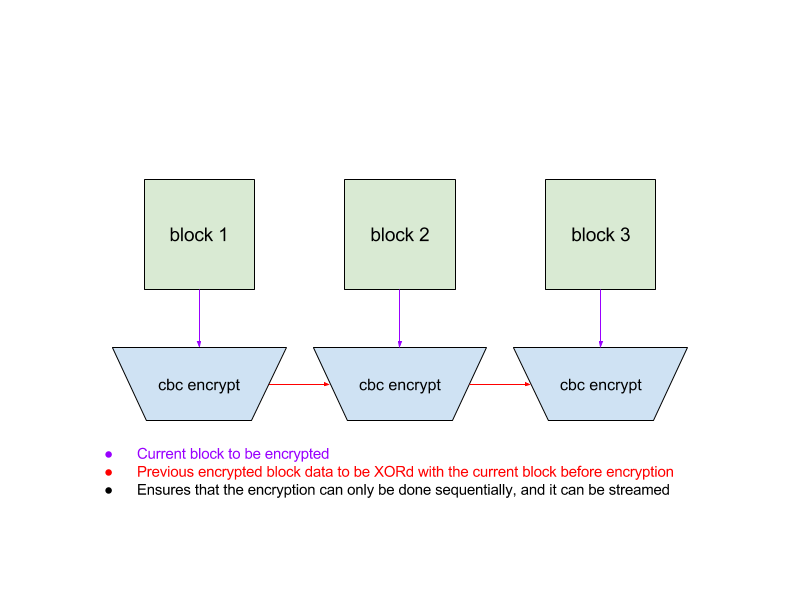
\includegraphics[width=0.6\textwidth]{../../figures/fig_7.png}
    \caption[図7]{シーケンシャルなCBCモード暗号化\label{fig:encrypt}}
  \end{center}
  \end{figure}

各データ複製ノードはPoHシーケンスのハッシュ値に署名することで固有の鍵を生成する。これはそれぞれの鍵と複製先ノード、PoHシーケンスを一意に組み合わせるので、特定のPoHシーケンスから発行されたハッシュ値を一意に選択できる。(ハッシュ値の選択についてはセクション\ref{hashselection}を参照)

すべてのデータセットはブロック毎に暗号化される。この鍵は各ブロックから32バイト分のサンプルを無作為に選び出すための擬似乱数のシードとして、PoRepの証明に利用される。

シーケンスから流れてきたPoHハッシュ値をCBCモードで暗号化した各ブロックの冒頭に繋げた値からマークルハッシュ値は計算される。

\begin{figure}
  \begin{center}
    \centering
    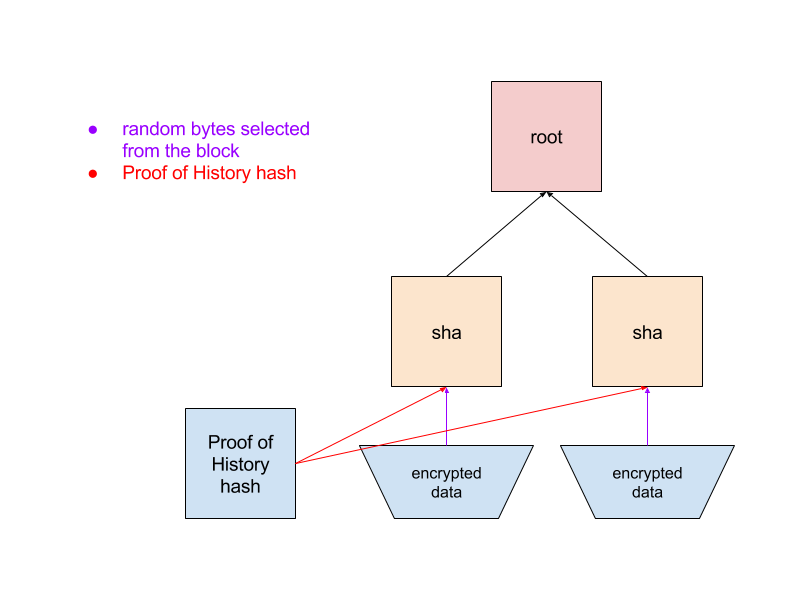
\includegraphics[width=0.6\textwidth]{../../figures/fig_8.png}
    \caption[図8]{高速なProof of Replication\label{fig_8}}
  \end{center}
  \end{figure}

ルートハッシュは鍵と一緒にPoHハッシュ値から発行される。データ複製ノードはPoHハッシュ値が発行されたとき、その時点からN回のハッシュ計算が行われるまでに証明を行わなくてはならない。ここで登場するNの値は、暗号化にかかる時間の約半分に相当するハッシュ計算回数を指す。PoH生成者は事前に決められた期間にProof of Replication用のハッシュ値を複数発行する。このときデータ複製ノードは証明に使うハッシュ値を選択する必要がある。これを一連の証明プロセスとし、完了後はハッシュ値の署名やルートハッシュ生成用のサンプリングから繰り返されることになる。

一定回数の証明を終えたとき、新しい鍵を使ってデータをCBCモードで改めて暗号化する。

\subsection{承認}

複数コアを利用して、各複製ノードを承認するための暗号化を並列かつブロックひとつひとつをこなすストリーム形式で計算することができる。必要な空き領域は合計で\(ブロック2個分 * コア数\)になり、これは各コア上で行われる今回ブロックの暗号化計算に、暗号化済み前回ブロックの値が必要なためである。各コアは暗号化済みブロックが使われる証拠すべての検証に使うことができる。

証拠の承認にかかる時間は暗号化計算にかかる時間におよそ等しい。ハッシュ計算の対象データのサイズを大きく削減するため、各ブロックから一部のバイト列を無作為にサンプリングする。同時に承認可能なデータ複製ノードの数は、利用可能なコアの数に等しい。現代のGPU3500以上のコアを備えるものの、CPUに比べてクロック速度が\(\frac{1}{2}\)〜\(\frac{1}{3}\)程度に劣る点に注意したい。

\subsection{鍵のローテーション}

鍵を切り替えないと同じ複製データから複数のPoHシーケンスに対し、陳腐化した証拠が生成される。よって鍵は周期的にローテーションされ、各複製データはそれぞれに特有のPoHシーケンスに紐付けられる新しい鍵で暗号化することにする。

現代のハードウェア構成では基本的に複製データの承認はGPU上で行われるで、そのクロック速度に合わせてローテーションの早さも調整する必要がある。

\subsection{ハッシュ値の選択}\label{hashselection}

PoH生成者はネットワーク全体がPoRepに使うハッシュ値を発行する。このハッシュ値は証明計算の高速化に必要なサンプリングの擬似乱数として使われる。

このハッシュ値は暗号化の計算にかかる約半分の時間に相当する周期で発行される。各データ複製ノードはそれぞれ同一ハッシュ値および暗号鍵を使い、またそのハッシュ値に署名した値をバイト列のサンプリングのシードとして使わなければならない。

各データ複製ノードは暗号化計算にかかるより短い時間内に複製データを保有している証拠を提出しなければならない。さもないとデータ複製ノードは暗号文をストリーム計算した上で、証明する度にデータ本体を削除できてしまう。

悪意のある生成者はハッシュ計算を行う直前に、ハッシュ値の操作を目的とした作為的なデータを挿入しようとするかもしれない。この攻撃への対処については\ref{subsubsec:collusion}で議論する。

\subsection{証拠の検証}
提供されたPoRepの証拠を検証する役割はPoHノードが担うものではない。データ複製ノードから提出された検証中あるいは承認済みの証拠を追跡可能にすることがPoHノードの役割である。データ複製ノードが提出した証拠に対する大多数の検証者からの署名を受けて、その証拠は正式に承認されたものとみなせる。

承認はデータ複製ノードによりP2Pゴシップネットワークで収集され、ネットワーク上の大多数の検証を含むパケットひとつで提出される。このパケットはPoHシーケンス上で特定ハッシュ値が発行される以前のすべての証拠を承認するもので、複数の複製データの承認を一度にできてしまう。

\subsection{攻撃}
\subsubsection{スパム}
高速な承認をすすめるためノードは承認を要求する際に、暗号化済みデータとマークル木全体をネットワークへ提供する仕様になっている。これを利用して、悪意のある利用者は多くのデータ複製ノードを作成し、PoRepに対する承認リクエストでネットワークを埋め尽くそうとするかもしれない。

本文におけるPoRepは複製された証拠の承認を安価にし、ネットワークの許容量を無駄に設計になっている。複製一件あたり1コアを、暗号計算に必要な時間分だけ専有されることになる。複製の最大許容数は利用可能な全コア数と同値にすべきである。現代のGPUでは3500個以上のコアを備える。

\subsubsection{部分消去}

データ複製ノードはデータ全部の保管を避けて、一部削除する可能性がある。証拠数に応じた試行回数とシードによる乱数値がこの攻撃を困難にする。

1テラバイト分のデータを保管するノードが、1メガバイトあたり1バイトのデータを削除するケースを想定する。1メガバイトあたり1バイトをサンプリングする証明を実施すると、削除部分と証拠部分が衝突する確率は\(1 - (1- 1/1,000,0000)^{1,000,000} = 0.63\)になる。証明を五回繰り返すだけで既に衝突する確率は99%を超えるため、部分削除の検知を避けることは極めて困難であると言える。

\subsubsection{PoH生成者との談合}

署名済みハッシュ値はサンプルの決定に使う擬似乱数のシード生成に使われる。もしデータ複製ノードが署名対象となるハッシュ値を事前に知ることができたら、サンプリングされない大部分のデータを削除できてしまう。

PoH生成者と談合しているデータ複製ノードはサンプリングに使われるハッシュ値が発行される直前のタイミングで特定の取引情報を挿し込む。十分に性能の高いコアが備えられていれば、攻撃者はデータ複製ノードにとって都合の良いハッシュ値を発行することもできる。

この攻撃は単体のデータ複製ノードにしか利益をもたらさない。すべてのノードはECDSA(あるいは相当の)計算で署名された同一ハッシュ値を使わなくてはならず、署名されたハッシュ値は各ノードに特有のものとなり衝突耐性を備える。結局この攻撃者はその談合ノードから生み出される僅かな利益しか得ることができない。

\subsubsection{DoS}
データ複製ノードを増やすコストは、ストレージを用意するコストに等しいと考えられる。一方でデータ複製ノードが増えたときに必要となる追加の計算能力は、ノード一つあたりCPUあるいはGPUの1コアとなる。

これはネットワーク上でデータ複製ノードを大量に作成することでDoS攻撃を実行できる可能性を示唆する。

合意プロトコルがデータ複製ノードを指名でき、可用性・帯域・配置などの面で適切な複製データから導かれる証拠のみを評価することで、この攻撃を制限することができる。

\subsubsection{コモンズの悲劇}

PoS承認者は検証を行わずに、PoRepから提供された証拠をひたすら承認する可能性がある。経済的インセンティブはPoS承認者たちに検証の実施を促す設計にすべきである。ひとつの対策として、PoS承認者とデータ複製ノードの間で採掘報酬を分け合う仕組みにする。

さらなる対策として、PoRep承認者が低確率で虚偽の証拠を提出する仕組みが考えられる。PoRep承認者は虚偽のデータを作ったプロセスを明かすことで、証拠が偽物だったことを証明することができる。PoS承認者が偽物の証拠を承認した場合、ただちにスラッシングで罰せられる。

\section{システムアーキテクチャ}\label{system_architecture}

\begin{figure}
  \begin{center}
    \centering
    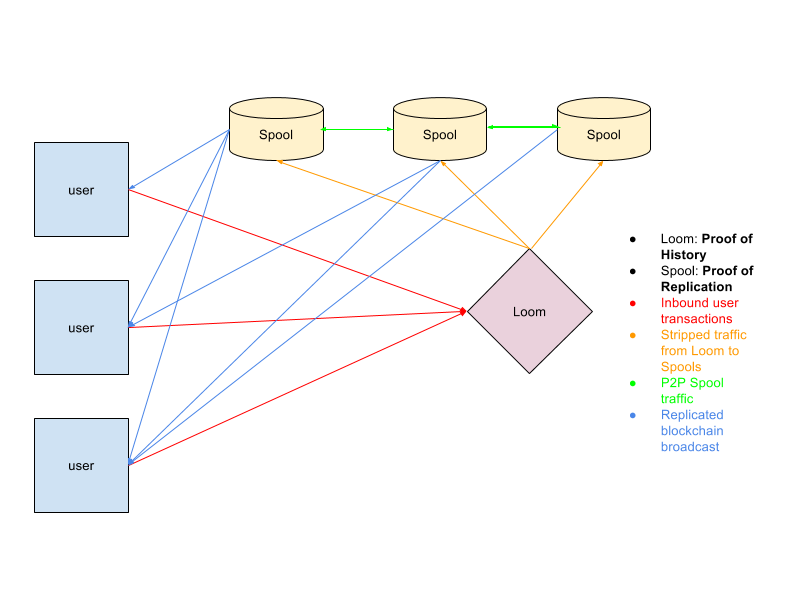
\includegraphics[width=0.6\textwidth]{../../figures/fig_9.png}
    \caption[Fig 9]{System Architecture \label{fig_9}}
  \end{center}
  \end{figure}

\subsection{Components}

\subsubsection{Leader, Proof of History generator}
The Leader is an elected Proof of History generator. It consumes arbitrary user transactions and outputs a Proof of History sequence of all the transactions that guarantees a unique global order in the system. After each batch of transactions the Leader outputs a signature of the state that is the result of running the transactions in that order. This signature is signed with the identity of the Leader.

\subsubsection{State}
A naive hash table indexed by the user’s address. Each cell contains the full user’s address and the memory required for this computation. For example\\
\noindent Transaction table contains:\\\\\noindent
\begin{bytefield}[bitwidth=.1em]{256}
\bitheader{0,31,63,95,127,159,191,223,255} \\
\bitbox{160}{Ripemd of Users Public Key}
& \bitbox{64}{Account}
& \bitbox{32}{unused}
\end{bytefield}\\
For a total of 32 bytes.\\
\noindent Proof of Stake bond’s table contains:\\\\\noindent
\begin{bytefield}[bitwidth=.1em]{256}
\bitheader{0,31,63,95,127,159,191,223,255} \\
\bitbox{160}{Ripemd of Users Public Key}
& \bitbox{64}{Bond} \\
& \bitbox{64}{Last Vote} \\
& \bitbox{224}{unused}
\end{bytefield}\\
For a total of 64 bytes.
\subsubsection{Verifier, State Replication}
The Verifier nodes replicate the blockchain state and provide high availability of the blockchain state. The replication target is selected by the consensus algorithm, and the validators in the consensus algorithm select and vote the Proof of Replication nodes they approve of based on off-chain defined criteria.

The network could be configured with a minimum Proof of Stake bond size, and a requirement for a single replicator identity per bond.
\subsubsection{Validators}
These nodes are consuming bandwidth from Verifiers. They are virtual nodes, and can run on the same machines as the Verifiers or the Leader, or on separate machines that are specific to the consensus algorithm configured for this network.

\subsection{Network Limits}

\begin{figure}
  \begin{center}
    \centering
    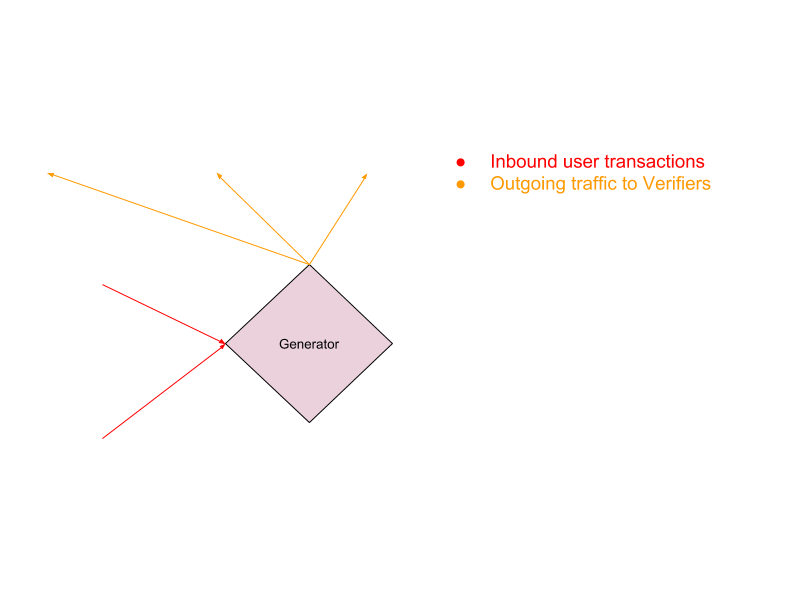
\includegraphics[width=0.8\textwidth]{../../figures/fig_10.png}
    \caption[Fig 10]{Generator network limits\label{fig_10}}
  \end{center}
  \end{figure}

Leader is expected to be able to take incoming user packets, orders them the most efficient way possible, and sequences them into a Proof of History sequence that is published to downstream Verifiers. Efficiency is based on memory access patterns of the transactions, so the transactions are ordered to minimize faults and to maximize prefetching.\\\\

\noindent Incoming packet format:\\\\\noindent
\begin{bytefield}[bitwidth=.1em]{256}
\bitheader{0,31,63,95,127,159,191,223,255} \\
\begin{rightwordgroup}{Signed}
\bitbox{160}{Last Valid Hash}
& \bitbox{64}{Counter}
& \bitbox{6}{u} 
& \bitbox{10}{s} \\
& \bitbox{64}{Fee} \\
& \bitbox{256}{From} \\
\end{rightwordgroup} \\
& \bitbox{256}{Signature 1 of 2} \\
& \bitbox{256}{Signature 2 of 2} \\
\end{bytefield}

\noindent Size \(20 + 8 + 16 + 8 + 32 + 32 32 = 148\) bytes.\\\\

The minimal payload that can be supported would be 1 destination account.
\noindent With payload:\\\\\noindent
\begin{bytefield}[bitwidth=.1em]{256}
\bitheader{0,31,63,95,127,159,191,223,255} \\
\begin{rightwordgroup}{Signed}
\bitbox{160}{Last Valid Hash}
& \bitbox{64}{Counter}
& \bitbox{6}{u}
& \bitbox{10}{s} \\ 
& \bitbox{160}{To}
& \bitbox{64}{Amount} \\
& \bitbox{64}{Counter}
& \bitbox{64}{Fee} \\
& \bitbox{256}{From} \\
\end{rightwordgroup} \\
& \bitbox{256}{Signature 1 of 2} \\
& \bitbox{256}{Signature 2 of 2} \\
\end{bytefield}

\noindent With payload the minimum size: 176 bytes\\\\

The Proof of History sequence packet contains the current hash, counter, and the hash of all the new messages added to the PoH sequence and the state signature after processing all the messages. This packet is sent once every N messages are broadcast.\\
\noindent Proof of History packet:\\\\\noindent
\begin{bytefield}[bitwidth=.1em]{256}
\bitheader{0,31,63,95,127,159,191,223,255} \\
\begin{rightwordgroup}{Signed}
\bitbox{160}{Current Hash}
& \bitbox{64}{Counter} \\
\bitbox{160}{Messages Hash} \\
\bitbox{160}{State Hash} \\
\end{rightwordgroup} \\
& \bitbox{256}{Signature 1 of 2} \\
& \bitbox{256}{Signature 2 of 2} \\
\end{bytefield}

\noindent Minimum size of the output packet is: 132 bytes \\\\

On a 1gbps network connection the maximum number of transactions possible is $1$~gigabit per second / $176$~bytes = $710$k tps max. Some loss $1-4\%$ is expected due to Ethernet framing. The spare capacity over the target amount for the network can be used to increase availability by coding the output with Reed-Solomon codes and striping it to the available downstream Verifiers.
\subsection{Computational Limits}
Each transaction requires a digest verification. This operation does not use any memory outside of the transaction message itself and can be parallelized independently. Thus throughput is expected to be limited by the number of cores available on the system.

GPU based ECDSA verification servers have had experimental results of 900k operations per second~\cite{gpuecc}.
\subsection{Memory Limits}
A naive implementation of the state as a \(50\%\) full hashtable with 32 byte entries for each account, would theoretically fit 10 billion accounts into 640GB. Steady state random access to this table is measured at \(1.1 * 10^7\) writes or reads per second. Based on 2 reads and two writes per transaction, memory throughput can handle 2.75m transactions per second. This was measured on an Amazon Web Services 1TB x1.16xlarge instance.

\subsection{High Performance Smart Contracts}\label{sec:smartcontracts}

Smart contracts are a generalized form of transactions. These are programs that run on each node and modify the state. This design leverages extended Berkeley Packet Filter bytecode as fast and easy to analyze and JIT bytecode as the smart contracts language.

One of its main advantages is a zero cost Foreign Function Interface. Intrinsics, or \hyphenation{high level} functions that are implemented on the platform directly, are callable by \hyphenation{user supplied} programs. Calling the intrinsics suspends that program and schedules the intrinsic on a high performance server. Intrinsics are batched together to execute in parallel on the GPU.

\begin{figure}
  \begin{center}
    \centering
    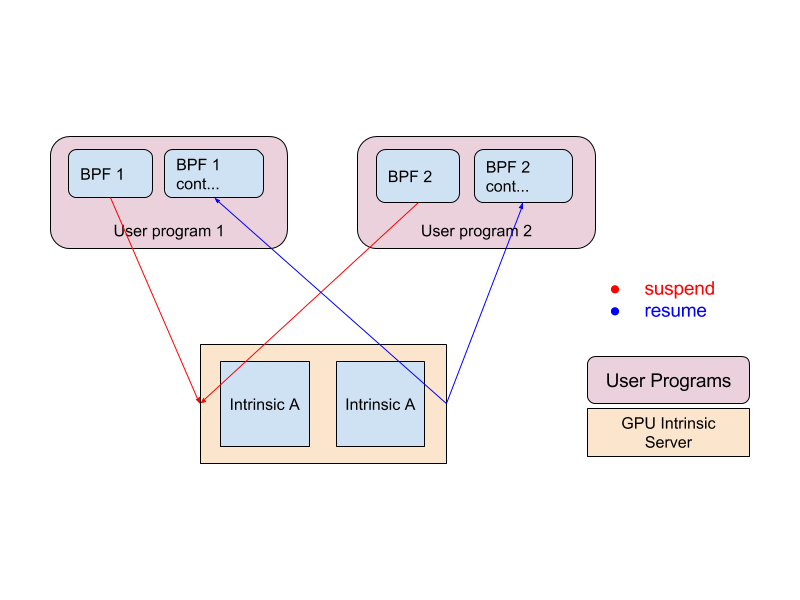
\includegraphics[width=0.6\textwidth]{../../figures/fig_11.png}
    \caption[Fig 11]{Executing \hyphenation{user supplied} BPF programs.\label{fig_11}}
  \end{center}
  \end{figure}

In the above example, two different user programs call the same intrinsic. Each program is suspended until the batch execution of the intrinsics is complete. An example intrinsic is ECDSA verification. Batching these calls to execute on the GPU can increase throughput by thousands of times.

This trampoline requires no native operating system thread context switches, since the BPF bytecode has a well defined context for all the memory that it is using.

eBPF backend has been included in LLVM since 2015, so any LLVM frontend language can be used to write smart contracts. It’s been in the Linux kernel since 2015, and the first iterations of the bytecode have been around since 1992. A single pass can check eBPF for correctness, ascertain its runtime and memory requirements and convert it to x86 instructions.

\bibliographystyle{abbrv}
\bibliography{simple}

\begin{thebibliography}{9}
\bibitem{liskov}
Liskov, Practical use of Clocks
\\\texttt{ http://www.dainf.cefetpr.br/~tacla/SDII/PracticalUseOfClocks.pdf}

\bibitem{spanner}
Google Spanner TrueTime consistency
\\\texttt{ https://cloud.google.com/spanner/docs/true-time-external-consistency}

\bibitem{ordering}
Solving Agreement with Ordering Oracles
\\\texttt{ http://www.inf.usi.ch/faculty/pedone/Paper/2002/2002EDCCb.pdf}

\bibitem{tendermint}
Tendermint: Consensus without Mining
\\\texttt{https://tendermint.com/static/docs/tendermint.pdf}

\bibitem{hashgraph}
Hedera: A Governing Council \& Public Hashgraph Network
\\\texttt{https://s3.amazonaws.com/hedera-hashgraph/hh-whitepaper-v1.0-180313.pdf}

\bibitem{filecoinporep}
Filecoin, proof of replication,
\\\texttt{https://filecoin.io/proof-of-replication.pdf}

\bibitem{slasher}
Slasher, A punative Proof of Stake algorithm
\\\texttt{https://blog.ethereum.org/2014/01/15/slasher-a-punitive-proof-of-stake-algorithm/}

\bibitem{delegatedpos}
BitShares Delegated Proof of Stake
\\\texttt{https://github.com/BitShares/bitshares/wiki/Delegated-Proof-of-Stake}

\bibitem{gpuecc}
An Efficient Elliptic Curve Cryptography Signature Server With GPU Acceleration
\\\texttt{http://ieeexplore.ieee.org/document/7555336/}

\bibitem{casper}
Casper the Friendly Finality Gadget
\\\texttt{https://arxiv.org/pdf/1710.09437.pdf}
\end{thebibliography}
\end{document}
This is never printed
